\documentclass[ex]{exercise_4.1}

\deadline{03.07.2024}

\begin{document}

\section{Van-der-Waals-Wechselwirkung}
{\it Die Anziehung zwischen zwei Molekülen werde durch die Van-der-Waals-Kräfte beschrieben. Untersuchen Sie die Abstandsabhängigkeit dieser Kräfte! Betrachten Sie ein Molekül mit einem Dipolmoment $\v p$, das entlang
der $x$-Achse ausgerichtet ist.}

\subsection{Wie hängt das von  einem Dipol hervorgerufene elektrische Feld vom Abstand \(x\) entlang der Dipolachse ab, wenn \(x\) groß gegenüber dem Dipolabstand ist?}

\dottedlinett

Die Bearbeitung der Aufgabe verwendet das CGS-Gauß-System. 
\begin{align*}
    \Delta \Phi(\v r ) &= -4\pi \rho(\v r)\\
    \implies \Phi(\v r) 
    &= \int \dV' \frac{\rho(\v r')}{\abs{\v r - \v r'}}\\
    &\approx \int \dV' \rho(\v r') \hug{\frac{1}{\abs{\v r - \v r'}}\eval_{\v r' =0}+\grad_{\v r'}\frac{1}{\abs{\v r - \v r'}}\eval_{\v r' =0}\cdot \v r'}\\
    &= \int \dV' \rho(\v r') \hug{\frac{1}{\absv r}+\frac{\v r\cdot \v r'}{\absv r^3}}\\
    &= \underbrace{\frac{Q}{r}}\sub{Monopol} + \underbrace{\frac{\v p \cdot \v r }{r^3}}\sub{Dipol} \with \begin{cases}
        Q = \int \dV \rho(\v r)\\
        \v p = \int \dV \v r \rho(\v r)
    \end{cases}\\
    \\
    \v E(\v r) &= -\grad \Phi(\v r) \\
    &= Q\frac{\v r}{r^3} +  \frac{3(\v p \cdot \v r)\v r}{r^5} - \frac{\v p }{r^3}\\
    &= \frac{Q \v r}{r^3} +  \frac{3(\v p \cdot \v r)\v r - \v p r^2}{r^5}\\
    \\
    Q=0, \v p = p \e_x:\ \v E(\v r) 
    &= \frac{3p (\e_x \cdot \v r)\v r - p \e_x r^2}{r^5}\\ 
    &= p\frac{3 x \v r - \e_x r^2}{r^5}\\ 
    \te{falls }\v r = x\e_x: \ &= \frac{2p}{x^3}\e_x
\end{align*}

\subsection{Betrachten Sie jetzt zusätzlich ein zweites, unpolarisiertes Molekül im Abstand \(x\), entlang der \(x\)-Achse. Berechnen Sie die proportionale Abhängigkeit der potenziellen Wechselwirkungsenergie der beiden Moleküle von ihrem Abstand \(x\) zueinander.}

\dottedlinett

\begin{align*}
    \Delta \Phi(\v r) &= -4\pi \rho(\v r)\\
    \rho(\v r) &= -\frac{1}{4\pi}\Delta \Phi(\v r)\\
    &= -\frac{1}{4\pi}\Delta \hug{\frac{\v p \cdot \v r }{r^3}}\\
    &= \frac{1}{4\pi}\Delta\hug{\v p\cdot \grad\hug{\frac{1}{r}}}\\
    &= \frac{1}{4\pi}\v p\cdot \grad \Delta \hug{\frac{1}{r}}\\
    &= \frac{1}{4\pi}\v p\cdot \grad \hug{-4\pi \delta(\v r)}\\
    &= -\v p\cdot \grad \delta(\v r)\\
    \\
    \v F 
    &= \int \dV \rho(\v r) \v E(\v r)\\
    &= -\v p\cdot  \int \dV \v E(\v r) \grad \delta(\v r)\\
    &= \v p\cdot  \int \dV \delta(\v r) \grad \v E(\v r) \\
    &= \v p\cdot \grad \v E \\
    \\
    \grad U &= -\v F\\ 
    &= -\v p\cdot \grad \v E\\
    \implies U  &= -\v p \cdot \v E
\end{align*}
\begin{align*}
    U\sub{ges} 
    &= U_1 + U_2\\
    &= -\v p\cdot \v E\sub{ind} -\v p\sub{ind}\cdot \v E\\
    &= -\v p \cdot \hug{-\frac{2p\sub{ind}}{x^3}\e_x} - \v p\sub{ind}\cdot \v E\\
    &= \v p \cdot \hug{\frac{2\alpha E}{x^3}\e_x} - (\alpha \cdot \v E)\cdot \v E\\
    &= \v p \cdot \hug{\frac{2\alpha}{x^3}\frac{2p}{x^3}\v e_x} - \alpha \frac{4p^2}{x^6}\\
    &= \frac{4\alpha p^2}{x^6} - \frac{4\alpha p^2}{x^6}\\
    &= 0
\end{align*}
Für mathematische Dipole (ohne räumliche Ausdehnung), eines mit intrinsischem und einem mit induziertem Dipolmoment, gibt es somit keine Wechselwirkung, wenn sie bereits die gleiche Ausrichtung haben, da sich beide Terme gegenseitig wegheben. Für ausgedehnte Dipole wie Molekülen ist dies nicht der Fall. Die Korrektur zu den beiden Termen, muss aber im Fernfeld nahtlos in den hier durchgerechneten Fall übergehen, weshalb man einen "{}educated guess"{} machen kann, dass für große \(x\) die Proportionalität \(U\sub{ges}\propto \frac{\alpha p^2}{x^6}\) gilt.   


\subsection{Berechnen Sie mit \(\v F=-\grad V\), die Proportionalität der Kraft zwischen den Molekülen zum Abstand \(x\).}

\dottedlinete

\begin{align*}
    \v F &= -\grad V \propto \grad \frac{\alpha p^2}{x^6} \propto \frac{\alpha p^2}{x^7} \\
\end{align*}

\section{}
{\it Die Größenordnung der Rotationsenergien relativ zu den elektronischen Energien im eV Bereich lässt sich aus einer semiklassischen Betrachtung und der Unschärferelation abschätzen. Man betrachte ein starres, zweiatomiges Molekül. Der quantenmechanische Ausdruck für die Energieniveaus aufgrund der Rotation dieses Systems lautet 
\begin{align*}
    E\sub{rot} = \frac{\hbar^2}{2\theta}j(j+1)
\end{align*}
wobei \(j\) die Rotationsquantenzahl bezeichnet.
}

\subsection{Zeigen Sie, das bei einer klassischen Betrachtung in der die Atome umeinander rotieren, das Trägheitsmoment \(\theta = \mu R^2\) ist, wobei \(\mu\) die reduzierte Masse und \(R\) den Atomabstand bezeichnet.}

\dottedlinett

Nach dem Satz von Steiner setzt sich das Trägheitsmoment \(\theta\) zusammen aus dem Trägheitsmoment im Schwerpunktsystem \(\theta_S\), der gesamt Masse \(M\) und dem Massenschwerpunkt \(\v R\): 
\begin{align*}
    \theta = \theta_S + M R^2\\
\end{align*}

Reduzierte Masse und Massenschwerpunkt sind jeweils gegeben durch 
\begin{align*}
    \mu &= \frac{m_1 m_2}{m_1 + m_2}\\
    \v R &= \mu\hug{\frac{\v r_1}{m_2} + \frac{\v r_2}{m_1}}
\end{align*}
Sei für die Berechnung von \(\theta_S\) die Rotationsachse \(\v \omega = \omega \e_z \), und \(\v r_{1}, \v r_{2}\in \Span\pug{\e_x, \e_y}\), d.h. es ist nur eine Haubtträgheitsachse von Interesse.

\begin{align*}
    \theta_S 
    &= m_1 \hug{\v r_1 -\v R}^2 + m_2 \hug{\v r_2 -\v R}^2\\
    &= m_1 \v r_1^2 + m_2 \v r_2^2 - 2(m_1 \v r_1 + m_2 \v r_2) \v R + (m_1+m_2)\v R^2\\
    &= m_1 \v r_1^2 + m_2 \v r_2^2 - 2 \mu (m_1 \v r_1 + m_2 \v r_2) \hug{\frac{\v r_1}{m_2} + \frac{\v r_2}{m_1}} + (m_1+m_2)\mu^2\hug{\frac{\v r_1}{m_2} + \frac{\v r_2}{m_1}}^2\\
    &= m_1 \v r_1^2 + m_2 \v r_2^2 - 2\mu \hug{\frac{m_1}{m_2}\v r_1^2  + 2 \v r_1 \v r_2 + \frac{m_2}{m_1}\v r_2^2} + (m_1+m_2)\mu^2\hug{\frac{\v r_1^2}{m_2^2} + \frac{\v r_2^2}{m_1^2} + 2\frac{\v r_1\v r_2}{m_1 m_2}}\\
    &= m_1 \v r_1^2 + m_2 \v r_2^2 - 2\mu \hug{\frac{m_1}{m_2}\v r_1^2  + 2 \v r_1 \v r_2 + \frac{m_2}{m_1}\v r_2^2} + \mu\hug{\frac{m_1}{m_2}r_1^2 + 2\v r_1\v r_2 + \frac{m_2}{m_1}\v r_2^2}\\
    &= m_1 \v r_1^2 + m_2 \v r_2^2 - \mu\hug{\frac{m_1}{m_2}\v r_1^2  + 2 \v r_1 \v r_2 + \frac{m_2}{m_1}\v r_2^2} \\
    &= m_1 \v r_1^2 + m_2 \v r_2^2 - \frac{m_1^2}{m_1+m_2}\v r_1^2  - 2 \mu \v r_1 \v r_2 - \frac{m_2^2}{m_1 + m_2}\v r_2^2 \\
    &= \hug{m_1- \frac{m_1^2}{m_1+m_2}}\v r_1^2  - 2 \mu \v r_1 \v r_2 + \hug{m_2-\frac{m_2^2}{m_1 + m_2}}\v r_2^2 \\
    &= \hug{\frac{m_1(m_1+m_2) -m_1^2 }{m_1+m_2}}\v r_1^2  - 2 \mu \v r_1 \v r_2 + \hug{\frac{m_2(m_1 + m_2) - m_2^2}{m_1 + m_2}}\v r_2^2 \\
    &= \mu \hug{\v r_1^2  - 2 \v r_1 \v r_2 + \v r_2^2 }\\
    &= \mu \hug{\v r_2 - \v r_1}^2
\end{align*}

\subsection{Zeichnen Sie das Niveauschema des starren Rotators für den Fall des $\schemie{CO}$-Moleküls ($R = 1.13 \A$) und
bestimmen Sie die Energie des ersten angeregten Zustandes. (Nehmen Sie ein Periodensystem der
Elemente zur Hilfe, um die Massen der Atome $\schemie C$ und $\schemie O$ herauszufinden.)}

\dottedlinett

Die Massen sind 
\begin{align*}
    m(\schemie C) &= \frac{12.011\E{-3}}{N_A}\u{kg} 
    = \SI{2.00e-26}{\kg}\\
    m(\schemie O) &= \frac{15.999\E{-3}}{N_A}\u{kg} 
    = \SI{2.66e-26}{\kg}\\
\end{align*}

Damit sind die Energieniveaus allgemein 
\begin{align*}
    E\sub{rot} 
    &= \frac{\v J^2}{2\theta}
    = \frac{j(j+1) \hbar^2}{2\mu R^2}\\
    &\approx j(j+1)\cdot \SI{239}{\micro\eV}\\
\end{align*}
und die Werte der untersten Niveaus sind:

\begin{center}
    \begin{tabular}{@{}lllllll@{}}
        \toprule
        \(j\): & 0&1&2&3&4&5\\
        $E\sub{rot}(j)$ in \(\u{meV}\):&0.0 & 0.477 & 1.43 & 2.86 & 4.77 & 7.16\\
        \bottomrule
    \end{tabular}
\end{center}

\begin{figure}[H]
    \centering
    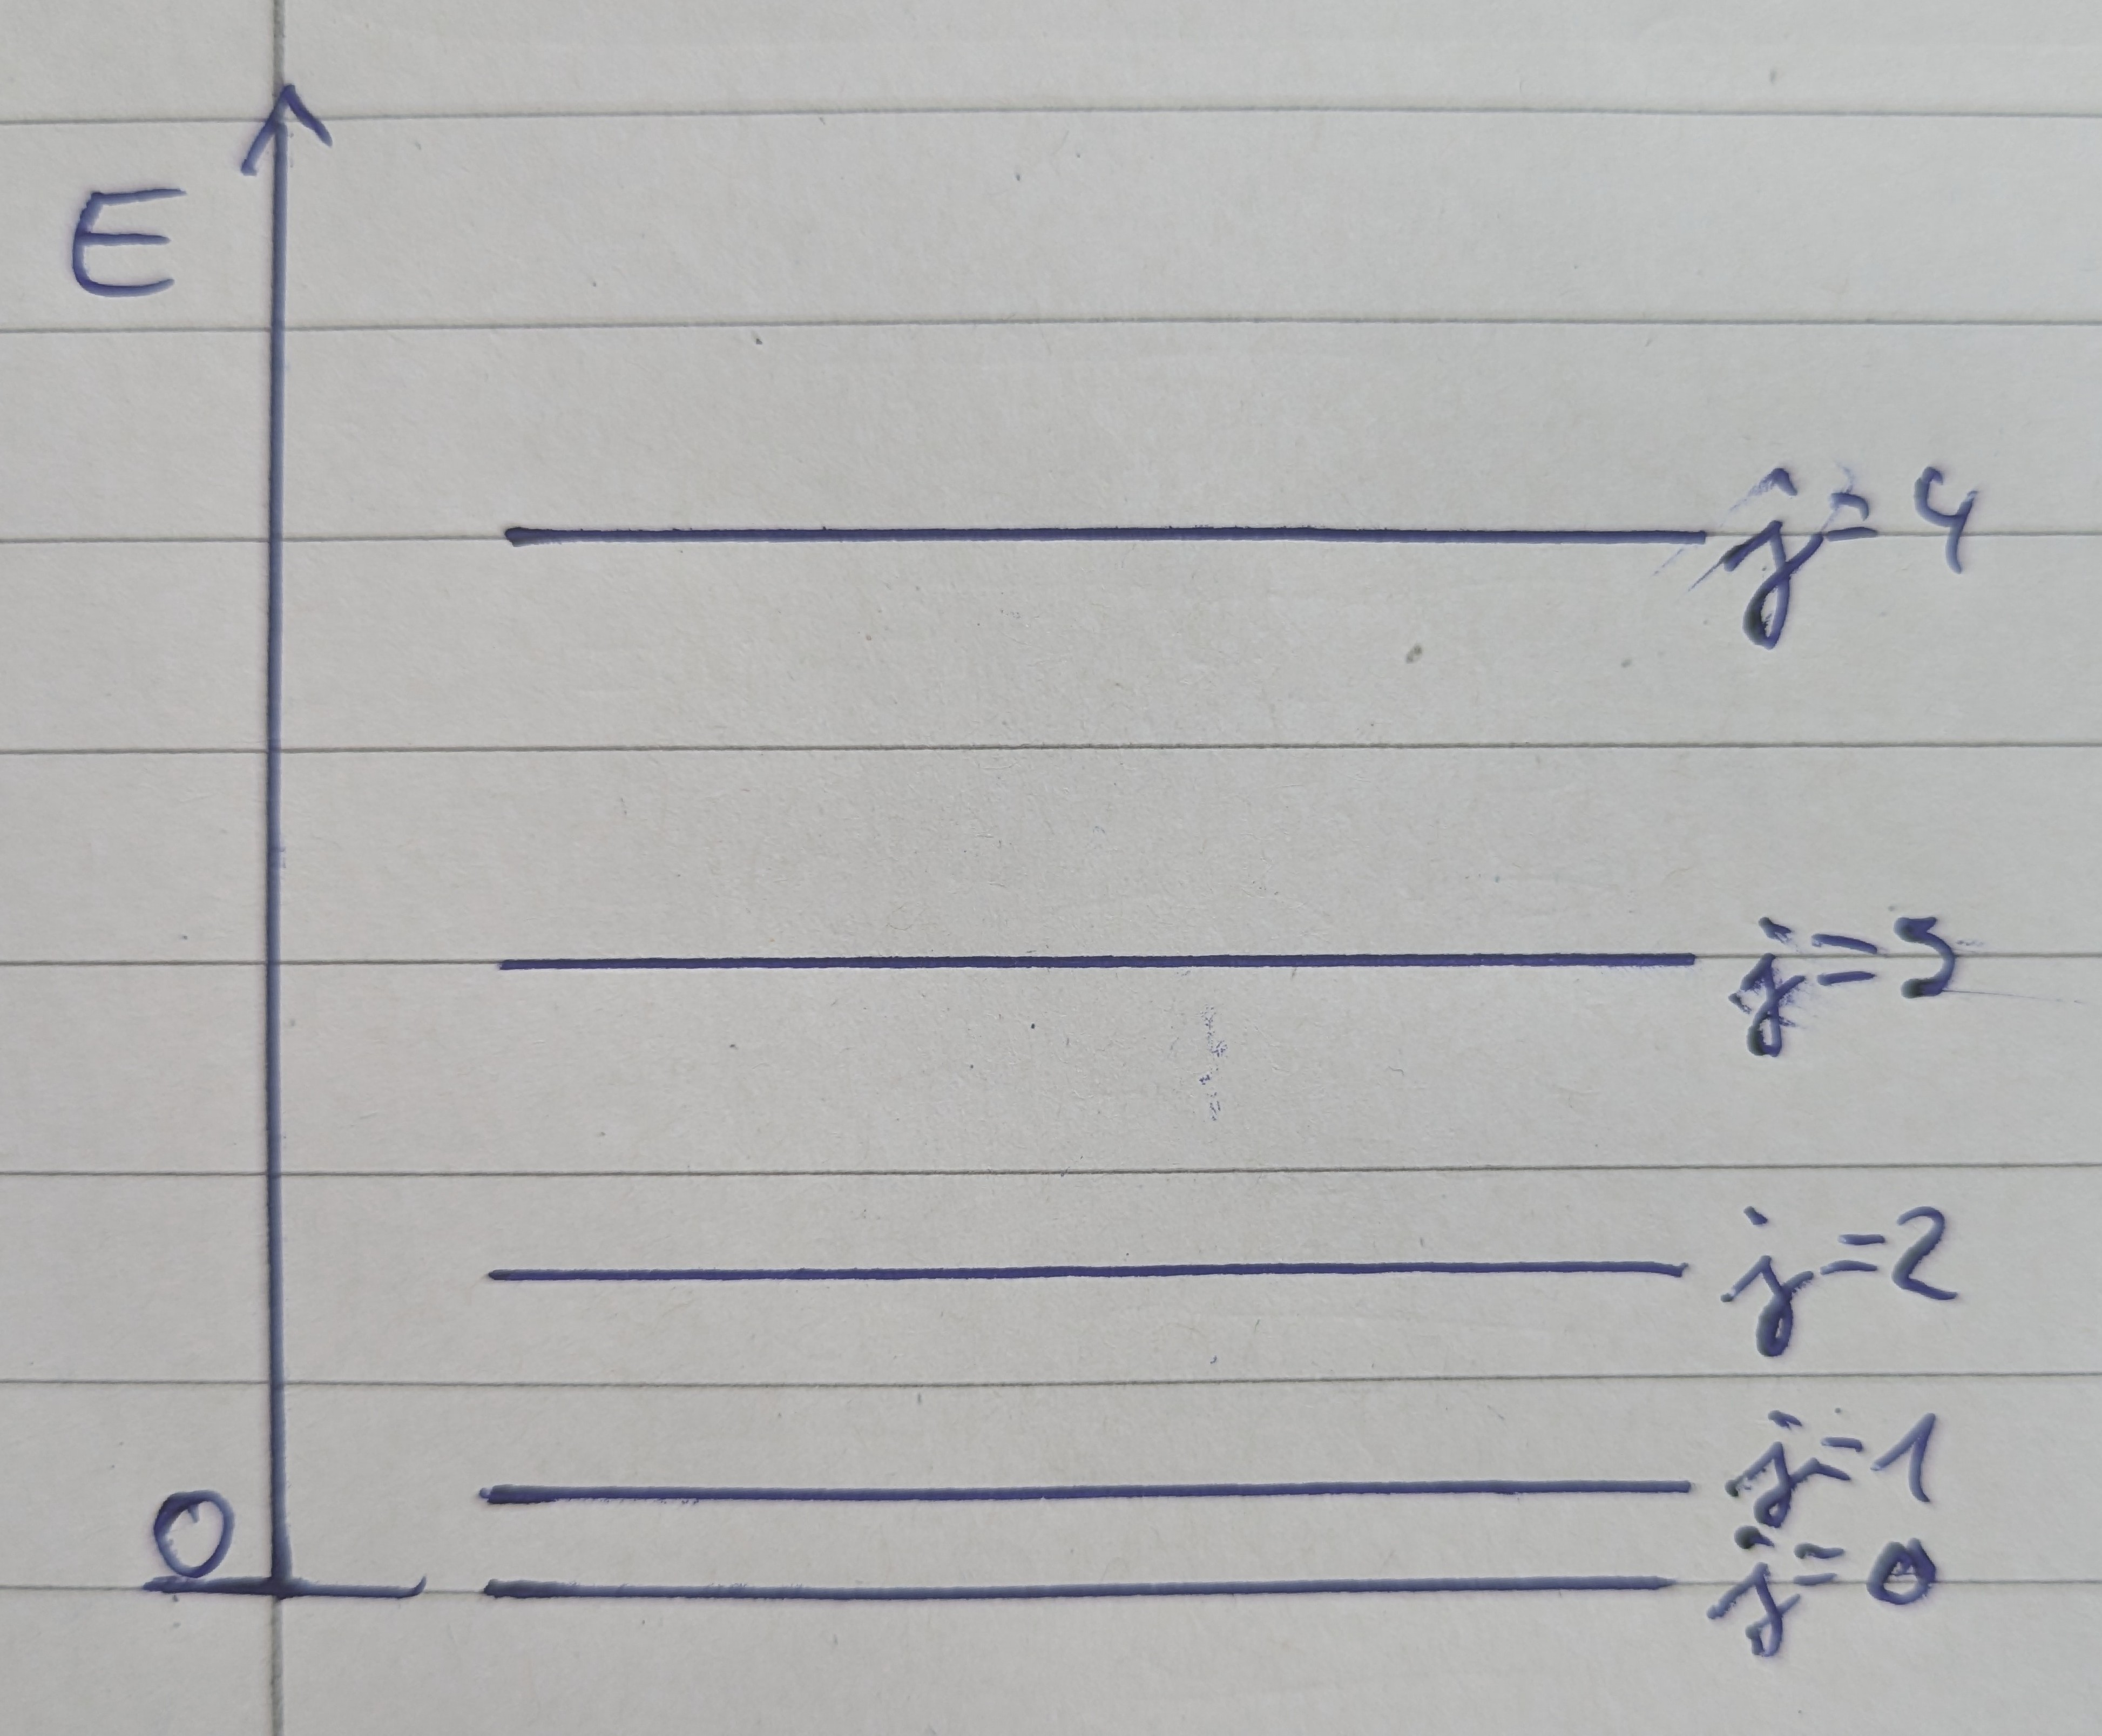
\includegraphics[width=0.6\textwidth]{j_energieniveaus.jpg}
    \caption{Skizze der Energieniveaus}
\end{figure}

\subsection{Rotationsbewegung eines $\schemie{H_2}$-Moleküls: Wie groß muss die Temperatur $T$ mindestens sein, damit die mittlere thermische Energie ausreicht, um den Zustand mit $J = 1$ anzuregen? (Abstand der $\schemie H$-Atome im $\schemie{H_2}$-Molekül: $0.75\A$.) Hinweis: Überlegen Sie sich die möglichen Freiheitsgrade für Bewegungen des Moleküls, die sich aus Translationen und möglichen Rotationen zusammensetzen.}

\dottedlinett

Es gibt in der Summe 5 Freiheitsgerade, drei für Translationen, einen für Schwingungen wie in (a) und einen weiteren für radiale Schwingungen um die Gleichgewichtslage.
Die mindest Temperatur ist daher 
\begin{align*}
    \tug{E\sub{th}} &\ge E\sub{rot}(j=1)\\
    \frac 52 k_B T &\ge \frac{j(j+1) \hbar^2}{2\mu R^2}\\
    T &\ge \frac{2\hbar^2}{5k_B \mu R^2}\\
    &= \frac{\hbar^2}{5k_B m_H R^2}\\
    &\approx \SI{7.54}{\K}
\end{align*}

\section{Schwingungsspektrum von \(\schemie{Li_2}\)}
{\it Das Schwingungsspektrum von Li$_2$ besteht aus Linien im Mikrowellenbereich, wobei der Abstand zweier benachbarter Linien jeweils $1.05 \cdot 10^{13}$ Hz beträgt. Berechnen Sie den Gleichgewichtsabstand der Bindungspartner in Li$_2$.}

\subsection{Nähern Sie zunächst das Molekülpotential im Minimum durch eine Parabel. Das Minimum des Potentials liegt beim Gleichgewichtsabstand $R_0$ und die Tiefe der Potentialmulde beträgt $E_D$. $E_D$ bezeichnet hierbei die Dissoziationsenergie und beträgt für Li$_2$ $1.10$ eV. Geben Sie das Potential an und diskutieren Sie die Form! Durch welche experimentelle Beobachtung kann die gefundene Form des Potentials bestätigt und damit die Näherung gerechtfertigt werden?}

\dottedlinete

\begin{align*}
    V(x) 
    &= \frac12\mu  \omega^2 (x- R_0)^2 - E_D
\end{align*}
Mit dem Parabelförmingen Potenzial hat man ein wohldefiniertes Minimum, jedoch sind die Grenzwerte für \(x\to \pm\inf\) inkorrekt, da diese gleich null sein müssten. Für kleine Auslenkungen aus der Gleichgewichtslage, sollte dies aber, nach dem Prinzip der Taylorentwicklung, eine gute Näherung sein. Experimentell kann die Form des Potenzials bestätigen, bzw. die Parameter bestimmen, indem man die Frequenzen der Übergange beobachtet. Für einen harmonischen Oszillator erwartete man einen konstanten Abstand \(\Delta f\) zwischen dem emittierten Frequenzen.

\subsection{Schätzen Sie die Größenordnung des Gleichgewichtsabstandes $R_0$ ab. Dieser entspricht der Amplitude $A$ eines harmonischen Oszillators bei dem die Vibrationsenergie $E\sub{vib} \approx E\sub D$, also in etwa der Dissoziationsenergie entspricht. \\
Bestimmen Sie damit einen Ausdruck für die "{}Federkonstante"{} des genäherten Potentials und bringen Sie diese in Relation mit der Schwingungsfrequenz, um auf $R_0$ zu schließen. \\
Hinweis: Um die Größenordnung des Gleichgewichtsabstandes $R_0$ abzuschätzen, nehmen Sie an, dass das Potential im Abstand von $\pm r_0/2$ vom Minimum auf die Hälfte seiner Tiefe (also auf den Wert $-E_D/2$) abgefallen ist. Alternativ können Sie sich überlegen, bei welchem Abstand das Molekül dissoziiert, also $V > 0$ gilt.}

\dottedlinett

\begin{align*}
    \Delta f &= \frac{\Delta E}{h} 
    = \frac{\hbar\omega }{h}
    = \frac{\omega}{2\pi}\\
    \omega &= 2\pi \Delta f \approx \SI{6.60E+13}{\Hz}\\
    k &= \mu \omega^2 = \frac12 m\sub{Li}\omega^2\approx \SI{25.0}{\kg\per\s^2}
\end{align*}

\begin{align*}
    E_D &\approx  \frac 12 k A^2 = \frac12 \mu\omega^2A^2 \\
    R_0&= A = \sqrt{\frac{2E_D}{\mu\omega^2}} \approx 1.19\A
\end{align*}
Der Literaturwert für \(R_0\) ist \(2.67\A\), somit stimmt die Größenordnung.

\section{Streuung von Deuteronen an Tritium}
{\it In einem Neutronengenerator werden Deuteronen $\hug{\schemie{^{2}_{1}H}}$ mit der Energie von $E = \SI{0.1}{\MeV}$  auf ein senkrecht zum Strahl stehendes Tritiumtarget $\hug{\schemie{^{3}_{1}H}}$ geschossen. In der Kernreaktion eines Deuteron mit einem Tritium wird jeweils ein freies Neutron erzeugt, das isotrop emittiert wird. Bei dieser Energie beträgt der Wirkungsquerschnitt für die Reaktion $8\u b$ . Das Tritiumtarget besitzt eine Flächenbelegungsdichte von $\rho_{F} = \rho \cdot d = \SI{0.2}{\mg\per\cm^2}$. Hierbei ist $\rho$ die Dichte des Materials und $d$ die Dicke des Targets.}

\subsection{Welcher Bruchteil der Neutronen erreicht einen $10 \times 10\u{cm}^{2}$ großen Detektor, der sich im Abstand von $5\u m $ hinter dem Produktionstarget befindet?}

\dottedlinete

\begin{align*}
    \alpha &\approx \frac{A\sub{D}}{4 \pi r^2} 
    \approx 0.0318\permil
\end{align*}

\subsection{Welchen Flussrate muss der Deuteronstrahl haben, damit auf dem Detektor eine Rate von $100$ Neutronen pro Sekunde eintrifft?\\
Hinweis: Nehmen Sie hierbei an, dass alle Neutronen ungestört und ohne weitere Wechselwirkung das Target verlassen und vernachlässigen Sie die Lebensdauer der Neutronen.}

\dottedlinete

\begin{align*}
    \sigma 
    &= \frac{1}{d \cdot \rho_T} \ln\hug{\frac{N_0}{N_0 - N\sub{Reaktion}}}\\
    &= \frac{M}{d N_A \rho} \ln\hug{\frac{N_0}{N_0 - N\sub{Reaktion}}}\\
    &= \frac{M}{N_A \rho_F} \ln\hug{\frac{N_0}{N_0 - N\sub{Reaktion}}}\\
    N_0 &= \exp\hug{\frac{\sigma N_A \rho_F}{M}}\hug{{N_0 - N\sub{Reaktion}}}\\
    &= -\frac{\exp\hug{\frac{\sigma N_A \rho_F}{M}}}{1 - \exp\hug{\frac{\sigma N_A \rho_F}{M}}} N\sub{Reaktion}\\
    &= \frac{N\sub{Reaktion}}{1-\exp\hug{-\frac{\sigma N_A \rho_F}{M}}} \\
    R_0 &= \frac{R\sub{Reaktion}}{1-\exp\hug{-\frac{\sigma N_A \rho_F}{M}}} \\
    &= \frac{R\sub{D}/\alpha}{1-\exp\hug{-\frac{\sigma N_A \rho_F}{M}}} \\
    &\approx \SI{1.96e10}{} 
\end{align*}
\end{document}